%% BioMed_Central_Tex_Template_v1.06
%%                                      %
%  bmc_article.tex            ver: 1.06 %
%                                       %

%%IMPORTANT: do not delete the first line of this template
%%It must be present to enable the BMC Submission system to
%%recognise this template!!

%%%%%%%%%%%%%%%%%%%%%%%%%%%%%%%%%%%%%%%%%
%%                                     %%
%%  LaTeX template for BioMed Central  %%
%%     journal article submissions     %%
%%                                     %%
%%          <8 June 2012>              %%
%%                                     %%
%%                                     %%
%%%%%%%%%%%%%%%%%%%%%%%%%%%%%%%%%%%%%%%%%


%%%%%%%%%%%%%%%%%%%%%%%%%%%%%%%%%%%%%%%%%%%%%%%%%%%%%%%%%%%%%%%%%%%%%
%%                                                                 %%
%% For instructions on how to fill out this Tex template           %%
%% document please refer to Readme.html and the instructions for   %%
%% authors page on the biomed central website                      %%
%% http://www.biomedcentral.com/info/authors/                      %%
%%                                                                 %%
%% Please do not use \input{...} to include other tex files.       %%
%% Submit your LaTeX manuscript as one .tex document.              %%
%%                                                                 %%
%% All additional figures and files should be attached             %%
%% separately and not embedded in the \TeX\ document itself.       %%
%%                                                                 %%
%% BioMed Central currently use the MikTex distribution of         %%
%% TeX for Windows) of TeX and LaTeX.  This is available from      %%
%% http://www.miktex.org                                           %%
%%                                                                 %%
%%%%%%%%%%%%%%%%%%%%%%%%%%%%%%%%%%%%%%%%%%%%%%%%%%%%%%%%%%%%%%%%%%%%%

%%% additional documentclass options:
%  [doublespacing]
%  [linenumbers]   - put the line numbers on margins

%%% loading packages, author definitions

%\documentclass[twocolumn]{bmcart}% uncomment this for twocolumn layout and comment line below
\documentclass{bmcart}

%%% Load packages
%\usepackage{amsthm,amsmath}
%\RequirePackage{natbib}
\RequirePackage{hyperref}
\usepackage[utf8]{inputenc} %unicode support
\usepackage{lscape}
\usepackage{graphicx}
\usepackage{pdflscape}
%\usepackage[applemac]{inputenc} %applemac support if unicode package fails
%\usepackage[latin1]{inputenc} %UNIX support if unicode package fails


%%%%%%%%%%%%%%%%%%%%%%%%%%%%%%%%%%%%%%%%%%%%%%%%%
%%                                             %%
%%  If you wish to display your graphics for   %%
%%  your own use using includegraphic or       %%
%%  includegraphics, then comment out the      %%
%%  following two lines of code.               %%
%%  NB: These line *must* be included when     %%
%%  submitting to BMC.                         %%
%%  All figure files must be submitted as      %%
%%  separate graphics through the BMC          %%
%%  submission process, not included in the    %%
%%  submitted article.                         %%
%%                                             %%
%%%%%%%%%%%%%%%%%%%%%%%%%%%%%%%%%%%%%%%%%%%%%%%%%


% \def\includegraphic{}
% \def\includegraphics{}



%%% Put your definitions there:
\startlocaldefs
\endlocaldefs


%%% Begin ...
\begin{document}

%%% Start of article front matter
\begin{frontmatter}

\begin{fmbox}
\dochead{Research}

%%%%%%%%%%%%%%%%%%%%%%%%%%%%%%%%%%%%%%%%%%%%%%
%%                                          %%
%% Enter the title of your article here     %%
%%                                          %%
%%%%%%%%%%%%%%%%%%%%%%%%%%%%%%%%%%%%%%%%%%%%%%

\title{SuperPhy: Predictive genomics for priority food-borne pathogens}

%%%%%%%%%%%%%%%%%%%%%%%%%%%%%%%%%%%%%%%%%%%%%%
%%                                          %%
%% Enter the authors here                   %%
%%                                          %%
%% Specify information, if available,       %%
%% in the form:                             %%
%%   <key>={<id1>,<id2>}                    %%
%%   <key>=                                 %%
%% Comment or delete the keys which are     %%
%% not used. Repeat \author command as much %%
%% as required.                             %%
%%                                          %%
%%%%%%%%%%%%%%%%%%%%%%%%%%%%%%%%%%%%%%%%%%%%%%

\author[
   addressref={aff1},                   % id's of addresses, e.g. {aff1,aff2}                      % id of corresponding address, if any
   noteref={n1},                        % id's of article notes, if any
   email={matthew.whiteside@phac-aspc.gc.ca}   % email address
]{\inits{MD}\fnm{Matthew D} \snm{Whiteside}}
\author[
   addressref={aff1},
   email={chad.r.laing@phac-aspc.gc.ca},
   noteref={n1}
]{\inits{CR}\fnm{Chad R} \snm{Laing}}
\author[
  addressref={aff1},
  email={akiff.manji@phac-aspc.gc.ca}
]{\inits{A}\fnm{Akiff} \snm{Manji}}
\author[
  addressref={aff1},
  email={peter.kruczkiewicz@phac-aspc.gc.ca}
]{\inits{P}\fnm{Peter} \snm{Kruczkiewicz}}
\author[
  addressref={aff1},
  email={eduardo.taboada@phac-aspc.gc.ca}
]{\inits{EN}\fnm{Eduardo N} \snm{Taboada}}
\author[
  addressref={aff1},
  email={vic.gannon@phac-aspc.gc.ca},
  corref={aff1}, 
]{\inits{VPJ}\fnm{Victor PJ} \snm{Gannon}}


%%%%%%%%%%%%%%%%%%%%%%%%%%%%%%%%%%%%%%%%%%%%%%
%%                                          %%
%% Enter the authors' addresses here        %%
%%                                          %%
%% Repeat \address commands as much as      %%
%% required.                                %%
%%                                          %%
%%%%%%%%%%%%%%%%%%%%%%%%%%%%%%%%%%%%%%%%%%%%%%

\address[id=aff1]{%                           % unique id
  \orgname{Laboratory for Foodborne Zoonoses, Public Health Agency of Canada}, % university, etc
  \street{Twp Rd 9-1},                     %
  \postcode{T1J 3Z4}                                % post or zip code
  \city{Lethbridge},                              % city
  \cny{Canada}                                    % country
}

%%%%%%%%%%%%%%%%%%%%%%%%%%%%%%%%%%%%%%%%%%%%%%
%%                                          %%
%% Enter short notes here                   %%
%%                                          %%
%% Short notes will be after addresses      %%
%% on first page.                           %%
%%                                          %%
%%%%%%%%%%%%%%%%%%%%%%%%%%%%%%%%%%%%%%%%%%%%%%

\begin{artnotes}
%\note{Sample of title note}     % note to the article
\note[id=n1]{Equal contributor} % note, connected to author
\end{artnotes}

\end{fmbox}% comment this for two column layout

%%%%%%%%%%%%%%%%%%%%%%%%%%%%%%%%%%%%%%%%%%%%%%
%%                                          %%
%% The Abstract begins here                 %%
%%                                          %%
%% Please refer to the Instructions for     %%
%% authors on http://www.biomedcentral.com  %%
%% and include the section headings         %%
%% accordingly for your article type.       %%
%%                                          %%
%%%%%%%%%%%%%%%%%%%%%%%%%%%%%%%%%%%%%%%%%%%%%%

\begin{abstractbox}

\begin{abstract} % abstract
% \parttitle{First part title} %if any
% \parttitle{Second part title} %if any

Predictive genomics involves the translation of raw genome sequence data into an assessment of the phenotypes exhibited by the organism from which the genome came. These phenotypes can range from how well the organism is able to survive in a particular environment, such as high salt concentration, to whether the organism will cause severe human disease. Advances in DNA sequencing technology have created new opportunities in the field of predictive genomics, which has application to fields as diverse as clinical medicine and epidemiology, where performing real-time, genome-based surveillance and identification of phenotypic characteristics of pathogens may be life-saving and reduce costs to the health care system through improved diagnostic, prevention and treatment efforts.

New analytical tools and infrastructure are needed to analyze the raw genomic data generated by current sequencing technology, a task that is recognized as a challenge worldwide. Significant progress has been made in the development of generic tools that are broadly applicable to all microorganisms; however, a fundamental missing component is the ability to analyze this data in the context of organism-specific knowledge. This accumulated knowledge from decades of research can provide a meaningful interpretation and context for the data. 

In this study, we have implemented an online predictive genomics platform
(http://lfz.corefacility.ca/superphy/) for \textit{Escherichia coli}. The platform integrates the analyses tools and genome sequence data for all publicly available genomes and facilitate the upload of genome sequences from users under public or private settings. The predictive genomics platform provides near real-time analyses of thousands of genome sequences using novel computational approaches with results that are understandable and useful to a wide community, including those in the fields of clinical medicine, epidemiology, ecology, and evolution. Specific analyses include identification of: 1) virulence and antimicrobial resistance determinants 2) epidemiological associations between specific genotypes, biomarkers, geospatial distribution, host, source, and other meta-data; 3) statistically significant clade-specific genome markers (presence / absence of specific genomic regions, and single-nucleotide polymorphisms) in bacterial populations; 4) \textit{in silico} molecular type for traditional wet-lab typing methods including Shiga-toxin subtyping.

\end{abstract}

%%%%%%%%%%%%%%%%%%%%%%%%%%%%%%%%%%%%%%%%%%%%%%
%%                                          %%
%% The keywords begin here                  %%
%%                                          %%
%% Put each keyword in separate \kwd{}.     %%
%%                                          %%
%%%%%%%%%%%%%%%%%%%%%%%%%%%%%%%%%%%%%%%%%%%%%%

\begin{keyword}
\kwd{sample}
\kwd{article}
\kwd{author}
\end{keyword}

% MSC classifications codes, if any
%\begin{keyword}[class=AMS]
%\kwd[Primary ]{}
%\kwd{}
%\kwd[; secondary ]{}
%\end{keyword}

\end{abstractbox}
%
%\end{fmbox}% uncomment this for twcolumn layout

\end{frontmatter}

%%%%%%%%%%%%%%%%%%%%%%%%%%%%%%%%%%%%%%%%%%%%%%
%%                                          %%
%% The Main Body begins here                %%
%%                                          %%
%% Please refer to the instructions for     %%
%% authors on:                              %%
%% http://www.biomedcentral.com/info/authors%%
%% and include the section headings         %%
%% accordingly for your article type.       %%
%%                                          %%
%% See the Results and Discussion section   %%
%% for details on how to create sub-sections%%
%%                                          %%
%% use \cite{...} to cite references        %%
%%  \cite{koon} and                         %%
%%  \cite{oreg,khar,zvai,xjon,schn,pond}    %%
%%  \nocite{smith,marg,hunn,advi,koha,mouse}%%
%%                                          %%
%%%%%%%%%%%%%%%%%%%%%%%%%%%%%%%%%%%%%%%%%%%%%%

%%%%%%%%%%%%%%%%%%%%%%%%% start of article main body
% <put your article body there>

%%%%%%%%%%%%%%%%
%% Background %%
%%
\section*{Introduction}
Predictive genomics involves the translation of whole-genome sequence data into an assessment of the phenotypes exhibited by the organism from which the genome came. Whole-genome sequencing (WGS) of bacterial isolates is now routinely employed in outbreak investigations and basic science research \cite{reuter_pilot_2013,fittipaldi_integrated_2013}. Currently a small number of organizations are employing WGS as part of routine surveillance efforts \cite{zankari_genotyping_2013,cody_real-time_2013}, such as Public Health England in its comprehensive \textit{Salmonella} genome sequencing program. Obtaining WGS data and performing exploratory comparative analyses is now commonplace, but meaningful interpretation of the raw data, also known as predictive genomics, lags considerably behind these initial analyses \cite{sherry_outbreak_2013}.

Bioinformaticians are able to use the requisite analytical tools and typically have access to the required computer infrastructure to compare genomes; however, they often lack the organism-specific knowledge necessary to meaningfully interpret the data for end-users. Conversely, microbiologists often have organism-specific knowledge but lack the bioinformatics wherewithal to meaningfully interpret the WGS data. This leads to fragmented workflows, group-specific data silos, the re-computation of common analyses, and failures to make important discoveries that would benefit the full community of users. As such, the enormous potential benefits of WGS are often not realized.

This is unfortunate given the scientific and public health benefits of WGS in realms such as  the real-time investigation and source attribution of nosocomial infections \cite{ halachev_genomic_2014, harris_whole-genome_2013,graham_real-time_2014}, genomic surveillance and epidemiology \cite{cody_real-time_2013}, and population genomic studies \cite{nasser_evolutionary_2014,kopac_genomic_2014}. The transition of public health laboratories to WGS will in the end replace traditional typing methods, and enable the identification of isolate differences down to a single base \cite{grad_epidemiologic_2014}. Such resolution combined with metadata will allow elucidation of transmission dynamics and clarify outbreak investigations and source-traceback. Lastly, identifying biomarkers (genes and single nucleotide polymorphisms) for genomic groups associated with phenotypes such as environmental niches or frequency and severity of human disease become possible.

Some efforts have been made to automate complex bioinformatics workflows, such as Taverna \cite{lanzen_taverna_2008} and Galaxy \cite{goecks_galaxy:_2010}, and while they are effective at simplifying the process, data are not integrated with these tools requiring users to transfer genome sequences from public or private databases and perform their own separate analyses. Likewise, online repositories of genome sequence data such GenBank at the National Center for Biotechnology Information \cite{benson_genbank_2012} and the Genomes Online Database \cite{pagani_genomes_2012} provide a wealth of data, but are decoupled from an efficient analytical platform.

Only recently have platforms emerged that attempt to provide both large-scale data storage and analyses. Relevant to microbiology, MicroScope and PATRIC provide broad pre-computed analyses for public genomes  \cite{vallenet_microscope--integrated_2012,wattam_patric_2013}. The Integrated Microbial Genomes (IMG) project is a combined genome annotation and analysis platform and allows for genomic data submission by the user \cite{markowitz_img_2013}. The Harvest suite of tools allows for fast core-genome alignments and interactive visualizations for thousands of genomes \cite{treangen_rapid_2014}.

Other platforms are organism specific, such as Sybil; a platform for the comparative analyses of \textit{Streptococcus pneumoniae} based on BLASTP searches \cite{riley_using_2012}. Outside of these broad analyses suites, other large-scale genome tools tend to focus on a specific analysis. For example, several tools provide a global phylogenetic tree for public bacterial genomes \cite{letunic_interactive_2011,fang_daily-updated_2013,federhen_ncbi_2011}.  

Several large WGS data analyses platforms are currently being developed world-wide, such as the Global Microbial Identifier project \url{http://www.globalmicrobialidentifier.org/}. These platforms take a very comprehensive approach and will be extremely useful in providing broad-based genome sequence analyses for all microbes of public health interest. These large projects promise to revolutionize molecular epidemiology. However, the outputs of these platforms out of necessity are very generic in nature and must be interpreted by species-specific experts for the data to be of use in answering specific biological questions. A recent study on outbreak investigations using WGS listed a main obstacle of routine adoption as `a paucity of user-friendly and clinically focused bioinformatics platforms'  \cite{sherry_outbreak_2013}. While some components necessary for phenotypic prediction based on WGS data have been developed, there is currently no single integrated platform built to provide predictive genomic analyses for organism-specific end-users.

We have previously developed Panseq, a suite of software tools that has allowed users to compare the genomes from a wide variety of bacteria \cite{laing_pan-genome_2010}. Using this program, the differences in the accessory genome and the single nucleotide variation in the core genome can be obtained and used to construct highly discriminatory and robust phylogenies. This ability to discriminate among groups of strains in turn allows inferences to be made quickly about the clonal spread of organisms in space and time, information that is invaluable in identifying and controlling sources of infections in disease outbreaks and the most important routes of sporadic disease transmission. 

Here we present Superphy, to bridge the gap between bioinformatics and organism-specific knowledge. SuperPhy incorporates discoveries from the decades of research on the pathogenesis and epidemiology of \textit{E. coli}, and translates the tremendous amount of data, genotypic and phenotypic, that have previously been generated into organism-specific knowledge. This knowledge is used in the SuperPhy predictive genomics platform to discover relationships among and about sub-groups that would otherwise be impossible. It allows non-bioinformaticians such as epidemiologists to quickly analyze new data against the background of all known \textit{E. coli}, allowing novel insights to be rapidly made.

Specific analyses include identification of: 1) virulence and antimicrobial resistance determinants 2) epidemiological associations between specific genotypes, biomarkers, geospatial distribution, host, source, and other meta-data; 3) statistically significant clade-specific genome markers (presence / absence of specific genomic regions, and single-nucleotide polymorphisms) in bacterial populations; 4) \textit{in silico} molecular type for traditional wet-lab typing methods including Shiga-toxin subtyping.

\section{Implementation}
\subsection{Webserver application and database}

Genome data and analyses are administered using a PostgreSQL 9.3 database with a schema adapted from the Generic Model Organism Database (GMOD) Chado schema \cite{mungall_chado_2007}. The Chado relational database schema uses a flexible, ontology-centric approach to organizing biological entities, relationships, properties and analysis. Entries in generic tables are assiged types using a mutable, controlled vocabulary. By not defining entity types directly into the relational layer, the database can be highly adaptable and can grow to add new analyses or biological data.

The application layer for the Superphy website is build using the Perl CGI Application framework, the RShiny framework and several public and custom Javascript libraries. The phylogenetic tree display and interaction is built on top of the Data Driven Documents (D3) JavaScript library. Geospatial views are built using the Google Maps JavaScript API v3 (\url{https://developers.google.com/maps/documentation/javascript/}). Group comparisons are processed and displayed using the RStudio Shiny web application framework for R \cite{racine_rstudio:_2012}.

The webserver application code base, database schema and public data are hosted at the following Github repository: ...

\subsubsection{Access to uploaded data}
Users can upload genomes and choose between three three access levels to govern use of their genome and meta data: `public', genome information is available to all users; `private', which allows the only the designated user and additional users they select, to use the uploaded genome data in online computation; and `private until a specified date', after which the data is released to `public'. Private data is accessible only to designated users, but can be combined with public data for user-specific analyses. Users can create custom strain-groups that can be saved, and all results may be download for offline analysis.

\subsection{Comparative genomic analyses}
Our previous pan-genomic analyses tool, Panseq is used for the background comparative analyses \cite{laing_pan-genome_2010}. It iteratively adds new genomic sequences, and compares them to those already stored in the platform. This computational approach allows a continuous influx of new sequence data without large time or memory requirements. In this way, the complete pan-genome of all sequences in the database is determined. Annotations for these regions are determined by querying the GenBank NR protein database via BLASTx.

differences in the accessory genome and the single nucleotide variation in the core genome are obtained and used by SuperPhy in downstream applications including the construction of highly discriminatory and robust phylogenies and providing the pre-computed data for biomarker identification between groups of genomes.

\subsubsection{Tree construction}
Phylogenies are created using a two-tier approach. Initially the presence / absence of the previously computed pan-genome is used to localize a new genome to a clade on the phylogenetic tree of all organisms with a fast relaxed neighbor-joining approach using Clearcut v.1.0.9 \cite{sheneman_clearcut:_2006}. The genomes in this clade and its parent are used to build a maximum likelihood tree with FastTreeMP under the GTR substitution model \cite{price_fasttree_2010}. Lastly, the ML tree of the clade and parent-clade of the new genome are combined using the scirpt X (github link) with the phylogeny of all the genomes in the database.

\subsubsection{Virulence and anti-microbial resistance markers}
The presence / absence of virulence and AMR genes, and single-nucleotide polymorphisms in shared genomic regions are automatically computed using Panseq. The non-redundant query set of AMR genes from the Comprehensive Antibiotic Resistance Database (CARD) \cite{mcarthur_comprehensive_2013} is used for \textit{in silico} AMR determinant screening. All AMR genes are organized and stored in the database according to their CARD-assigned Antibiotic Resistance Ontology annotation to aid in identifying the presence of different antimicrobial resistance mechanisms . The virulence gene database was constructed by obtaining all gene alleles of known virulence factors for \textit{E. coli} from the Virulence Factor Database \cite{chen_vfdb_2011}, supplemented with additional virulence factors from `\textit{Escherichia coli}: Pathotypes and Principles of Pathogenesis, 2nd Ed.' , and additional published literature \cite{donnenberg_escherichia_2013}. 

\subsubsection{Group comparisons}
The statistical identification of markers that differ between groups based on both single nucleotide polymorphisms and the presence / absence of genomic loci is implemented using Fisher’s Exact Test from the R statistical package \cite{r_foundation_for_statistical_computing_r:_2005}. All single-nucleotide polymorphisms and genomic presence / absence data reside in the database, requiring only the retrieval and P-value computation for the strains of interest, allowing for real time analysis.

The R Shiny interface is used for group creation and all metadata fields are pre-populated for all strains in the database. This makes comparing, for example, all human and non-human strains of a given serotype as simple as selecting groups based on the auto-filled serotype and host metadata fields, and clicking the compare button. Additionally, custom groups of any genomes can be created by any user, and saved to the user-profile so they become available whenever the user is logged in. These custom groups can include private genomes available only to the logged-in user.

\subsection{Continuous integration}
The user community will provide constant feedback as the platform evolves. A process of continuous integration will ensure that new innovations are implemented and optimizations applied based on the feedback.

\subsection{Maps}
Maps are one of the core visualization tools of Superphy and provide users with an interactive interface for obtaining and searching genomes with geospatial meta-information. Superphy has leveraged Google Maps along with their companion Javascript library, Google Maps API (V3), to provide a scalable method of interacting with thousands of genomes. 

Upon upload to SuperPhy, genomes with available isolation location meta-data are geocoded for their latitude and longitude. As there are thousands of genomes in the database with sometimes overlapping geospatial information, simply rendering each of the genome locations on the map would lead to a severe bottleneck in browser performance. Moreover, the utility as a visualization tool is degraded as map markers crowd the view port and become difficult to distinguish from one another.

To address these issues, we implemented marker clustering. Locations that fall within a distance of X from each other are clustered together into a single marker rendered at the geometric center of the cluster, and a count of the number of clustered locations is shown on the marker icon. As the user zooms in on the map the number of markers to display is reduced and individual locations re-materialize as single markers. 

As some genomes have identical isolation locations, their markers render at exactly the same coordinates on the map. Discerning genomes at these locations directly on the map is not currently feasible. As a result, maps are accompanied by a dynamic and sortable table of genome metadata that is by default sorted by Country. Users also have the option of sorting by Province, State and City. As users zoom in and out, and pan across the maps, the table changes to show only those genomes currently in the map view port. Isolation locations for each genome is also available for download in a tab delimited text file.

\section{Example Analyses}

\subsection{Pan-genome}
The proof-of-concept implementation of SuperPhy utilizes all publicly available \textit{E. coli} genome sequences from GenBank \cite{benson_genbank_2012}. \textit{E. coli} is ubiquitous, gram-negative bacterial species found in the intestines of healthy mammals, with only a small subset causing disease in humans or animals \cite{tenaillon_population_2010}. The population structure of \textit{E. coli} was initially described as being broadly distributed among four large and two smaller phylogenetic groups \cite{selander_methods_1986,goullet_comparative_1989}. Recent studies have found that the species has an open pan-genome, meaning that the addition of new genomes is likely to add additional genes to the pool \cite{medini_microbial_2005}. The pan-genome is highly variable, with around 80\% of an individual genome comprised of accessory genes, with the remainder from the shared core-genome \cite{lukjancenko_comparison_2010}; a stable proportion of approximately 4000 genes are present in at least 50\% of the genomes \cite{gordienko_evolution_2013}.

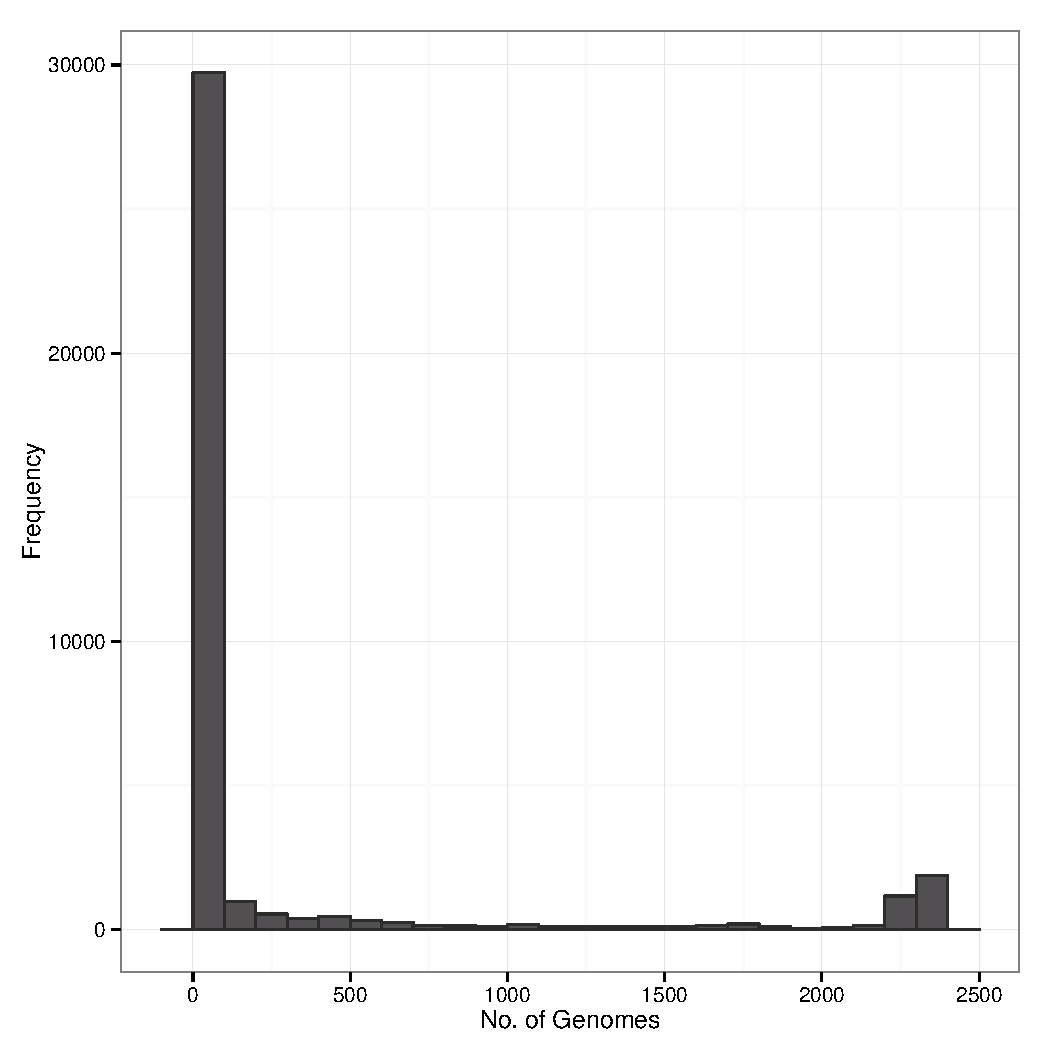
\includegraphics[width=\textwidth]{images/panGenomeSize.pdf}

The pan-genome distribution of the 2324 \textit{E. coli} genomes in the SuperPhy database as 1000bp genomic segments is presented in Figure X. As can be seen, the majority (29.7Mbp) of the 37.44 Mbp pan-genome is present in fewer than 100 genomes, with the core genome size (present in at least 2300 genomes) observed to be 1.86Mbp. Only 5.84Mbp of the pan-genome was found in greater than 100 genomes, but fewer than 2300 genomes.


%I think we can show VFs and group comparison via phylogenetic clade by replicating the study
%we can then do a separate for AMR, and possibly for GeoPhy as well
\subsection{Analyses of Hazen et al. (2013)}
Hazen et al. (2013) examined the attaching and effacing \textit{E. coli} (AEEC) using phylogenomic analyses of 144 genomes \cite{hazen_refining_2013}. By definition this group includes \textit{E. coli} capable of forming attaching and effacing lesions via the locus of enterocyte effeacement (LEE) \cite{croxen_recent_2013}. Within this large group are those \textit{E. coli} that also produce Shiga-toxin, forming the group known as enterohemorrhagic \textit{E. coli}, and those that do not produce Stx, known as  the enteropathogenic \textit{E. coli}, which themselves may or may not contain plasmid-encoded genes for the bundle-forming pilus.  The Hazen et al. (2013) study identified five distinct lineages of AEEC and examined the distribution of virulence factors associated with the AEEC group, notably genes encoding the LEE, Stx, and non-LEE encoded effector proteins. The study also identified regions that were over-represented or specific to each of the five lineages.

Using SuperPhy, the above analyses can be replicated. 
1) Select only LEE containing strains via VF (hmmm ... maybe we can't do this)
2) look at distribution of LEE, stx and effector proteins of strains
3) identify phylogeny (hopefully 5 lineages)
4) using group compare, create a group for each lineage
5) find markers for each group


\subsection{Anti-microbial resistance determinants}

\subsection{Group comparisons}

\subsection{Geospatial and phylogenetic concordance}
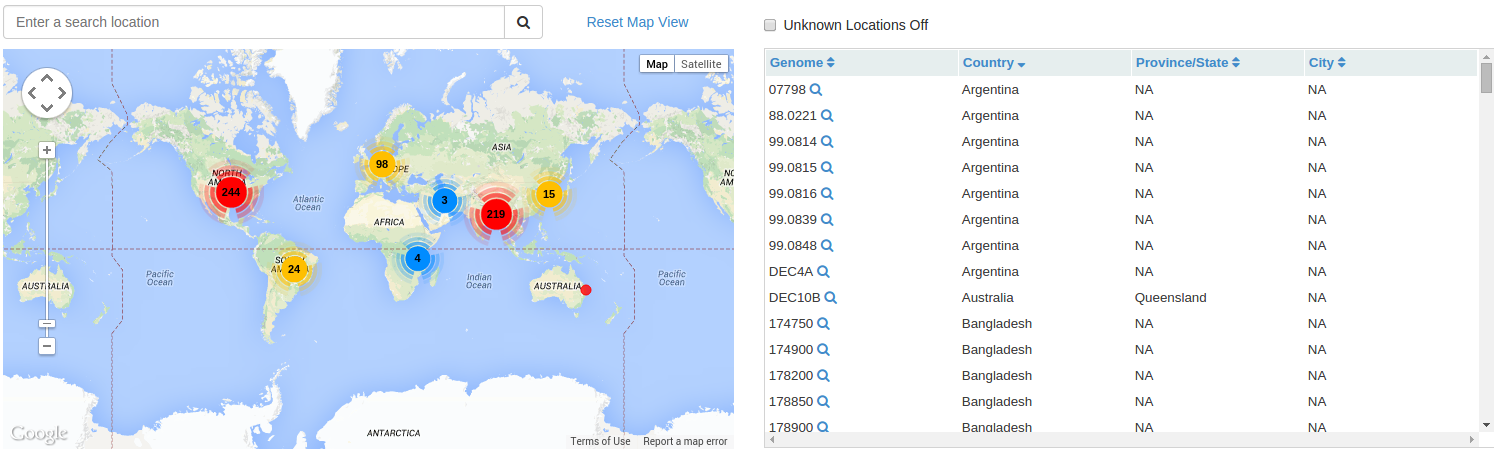
\includegraphics[width=\textwidth]{images/map.png}
Maps are highly integrated with the Superphy genome search and filtering controls, and this feature is designed to work seamlessly across all components of the website. The filtering system will only show map markers and genomes on the map table that are part of the filter / search query. Therefore, users can quickly and easily identify and select genomes with particular attributes, isolated from a region of interest, before querying additional information. Users can also add sortable metadata fields to the map table by selecting from the list of check boxes in the metadata side control panel. 

For ease of access, each map comes with a quick search that will pan and zoom to a location of interest. The accompanying map table will update the list of genomes currently in the map view port. As an example here we show the map when a user searches for `United Kingdom'.

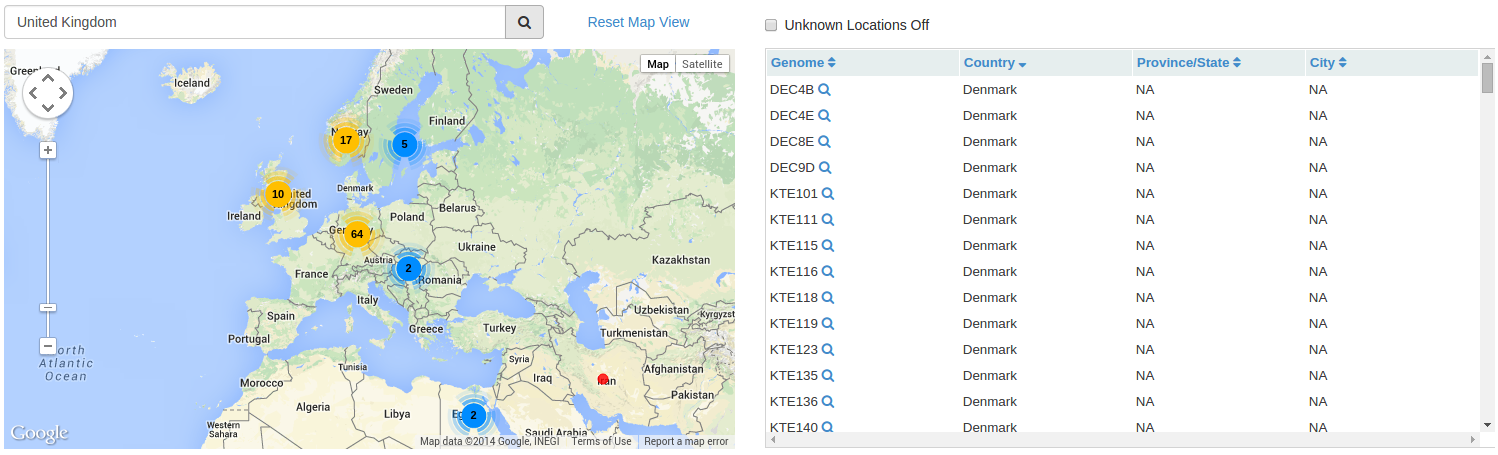
\includegraphics[width=\textwidth]{images/uk-map.png}

The interactive phylogenetic tree in SuperPhy is a powerful visual tool for discerning evolutionary relationships between genomes. The GeoPhy tab presents a synchronized tree and map within a single view, which allows users to view these evolutionary relationships across space and time, aiding in the answering of research and epidemiological questions.

As an example, a user can select a clade of genomes by clicking in the phylogenetic tree view and have these same strains mirrored in the geospatial view. Conversely, strains on the map can be selected and their phylogenetic relationship shown. Such visualizations can help determine whether a cluster of strains is potentially part of an outbreak, or help to determine the spread of particular genomic types across space and time.

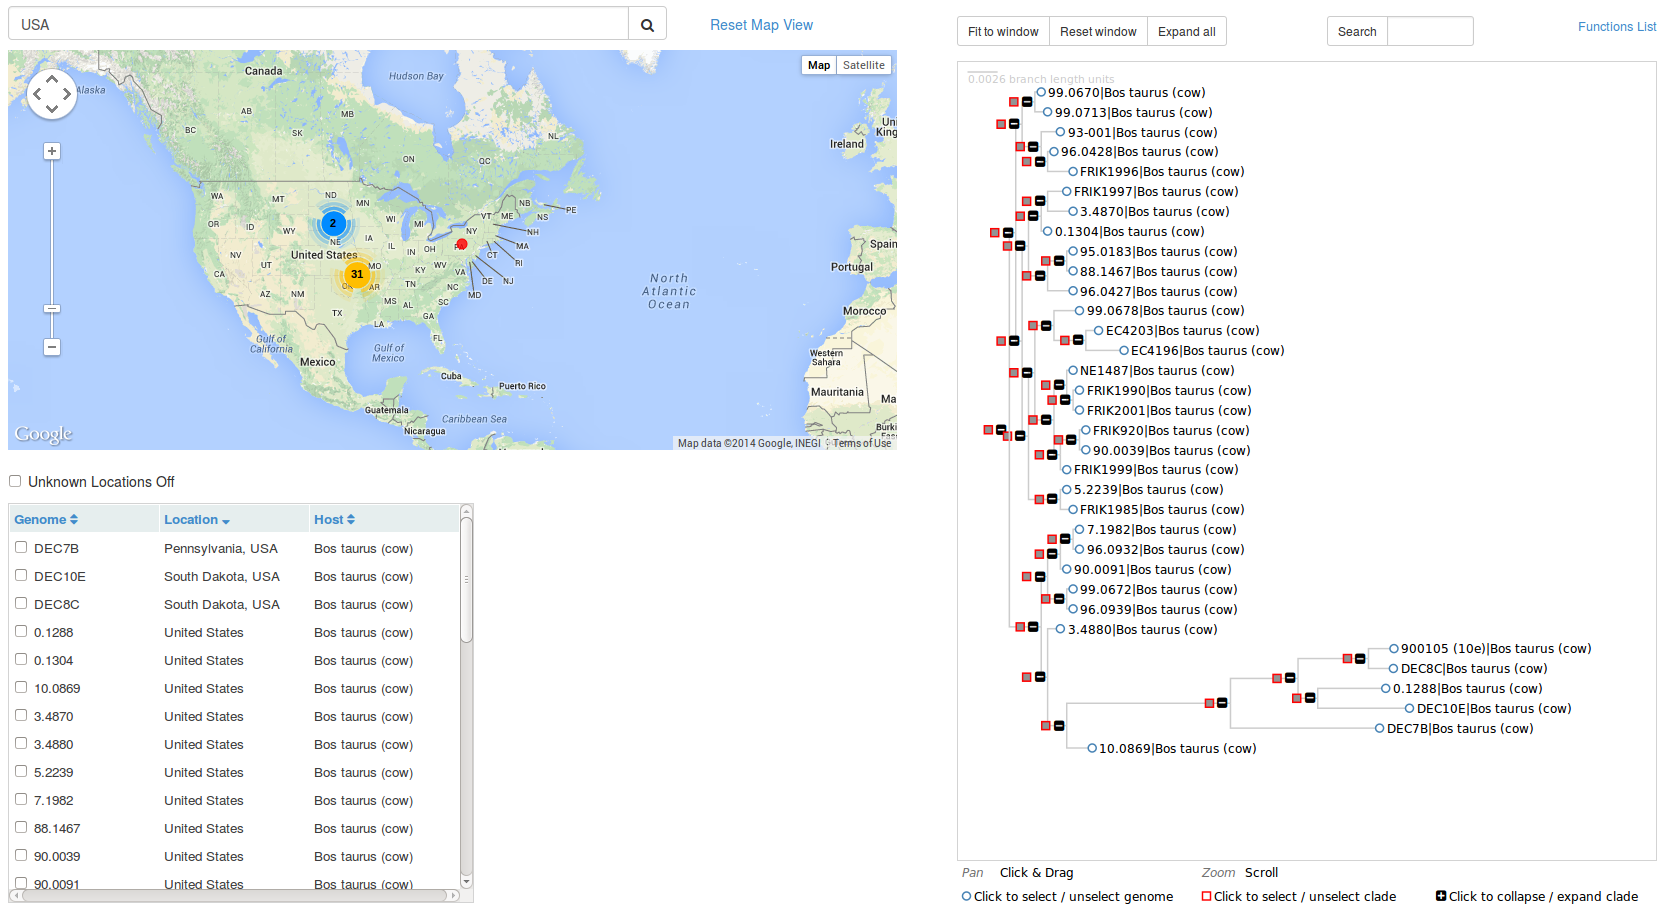
\includegraphics[width=\textwidth]{images/geophy.png}

\section{Conclusions}
SuperPhy allows users to identify genotypic clusters that vary in virulence and the statistically supported genetic elements responsible for these phenotypic differences. Predictive genomics is currently the missing translation layer between the vast amounts of information that many platforms are capable of producing, and true biological knowledge in a specific domain that is needed to test hypotheses.

% \subsection*{Sub-heading for section}
% Text for this sub-heading \ldots
% \subsubsection*{Sub-sub heading for section}
% Text for this sub-sub-heading \ldots
% \paragraph*{Sub-sub-sub heading for section}
% Text for this sub-sub-sub-heading \ldots
% In this section we examine the growth rate of the mean of $Z_0$, $Z_1$ and $Z_2$. In
% addition, we examine a common modeling assumption and note the
% importance of considering the tails of the extinction time $T_x$ in
% studies of escape dynamics.
% We will first consider the expected resistant population at $vT_x$ for
% some $v>0$, (and temporarily assume $\alpha=0$)
% %
% \[
%  E \bigl[Z_1(vT_x) \bigr]= E
% \biggl[\mu T_x\int_0^{v\wedge
% 1}Z_0(uT_x)
% \exp \bigl(\lambda_1T_x(v-u) \bigr)\,du \biggr].
% \]
% %
% If we assume that sensitive cells follow a deterministic decay
% $Z_0(t)=xe^{\lambda_0 t}$ and approximate their extinction time as
% $T_x\approx-\frac{1}{\lambda_0}\log x$, then we can heuristically
% estimate the expected value as
% %
% \begin{eqnarray}\label{eqexpmuts}
% E\bigl[Z_1(vT_x)\bigr] &=& \frac{\mu}{r}\log x
% \int_0^{v\wedge1}x^{1-u}x^{({\lambda_1}/{r})(v-u)}\,du
% \nonumber\\
% &=& \frac{\mu}{r}x^{1-{\lambda_1}/{\lambda_0}v}\log x\int_0^{v\wedge
% 1}x^{-u(1+{\lambda_1}/{r})}\,du
% \nonumber\\
% &=& \frac{\mu}{\lambda_1-\lambda_0}x^{1+{\lambda_1}/{r}v} \biggl(1-\exp \biggl[-(v\wedge1) \biggl(1+
% \frac{\lambda_1}{r}\biggr)\log x \biggr] \biggr).
% \end{eqnarray}
% %
% Thus we observe that this expected value is finite for all $v>0$ (also see \cite{koon,khar,zvai,xjon,marg}).



%%%%%%%%%%%%%%%%%%%%%%%%%%%%%%%%%%%%%%%%%%%%%%
%%                                          %%
%% Backmatter begins here                   %%
%%                                          %%
%%%%%%%%%%%%%%%%%%%%%%%%%%%%%%%%%%%%%%%%%%%%%%

\begin{backmatter}

\section*{Competing interests}
  The authors declare that they are competing for your interest.

\section*{Author's contributions}
    Text for this section \ldots

\section*{Acknowledgements}
  We would like to thank YOU, for reading this far.  \ldots
%%%%%%%%%%%%%%%%%%%%%%%%%%%%%%%%%%%%%%%%%%%%%%%%%%%%%%%%%%%%%
%%                  The Bibliography                       %%
%%                                                         %%
%%  Bmc_mathpys.bst  will be used to                       %%
%%  create a .BBL file for submission.                     %%
%%  After submission of the .TEX file,                     %%
%%  you will be prompted to submit your .BBL file.         %%
%%                                                         %%
%%                                                         %%
%%  Note that the displayed Bibliography will not          %%
%%  necessarily be rendered by Latex exactly as specified  %%
%%  in the online Instructions for Authors.                %%
%%                                                         %%
%%%%%%%%%%%%%%%%%%%%%%%%%%%%%%%%%%%%%%%%%%%%%%%%%%%%%%%%%%%%%

% if your bibliography is in bibtex format, use those commands:
\bibliographystyle{bmc-mathphys} % Style BST file
\bibliography{superphy_bmc_article}      % Bibliography file (usually '*.bib' )

% or include bibliography directly:
% \begin{thebibliography}
% \bibitem{b1}
% \end{thebibliography}

%%%%%%%%%%%%%%%%%%%%%%%%%%%%%%%%%%%
%%                               %%
%% Figures                       %%
%%                               %%
%% NB: this is for captions and  %%
%% Titles. All graphics must be  %%
%% submitted separately and NOT  %%
%% included in the Tex document  %%
%%                               %%
%%%%%%%%%%%%%%%%%%%%%%%%%%%%%%%%%%%

%%
%% Do not use \listoffigures as most will included as separate files

\section*{Figures}
  \begin{figure}[h!]
  \caption{\csentence{Sample figure title.}
      A short description of the figure content
      should go here.}
      \end{figure}

\begin{figure}[h!]
  \caption{\csentence{Sample figure title.}
      Figure legend text.}
      \end{figure}

%%%%%%%%%%%%%%%%%%%%%%%%%%%%%%%%%%%
%%                               %%
%% Tables                        %%
%%                               %%
%%%%%%%%%%%%%%%%%%%%%%%%%%%%%%%%%%%

%% Use of \listoftables is discouraged.
%%
\section*{Tables}
\begin{table}[h!]
\caption{Sample table title. This is where the description of the table should go.}
      \begin{tabular}{cccc}
        \hline
           & B1  &B2   & B3\\ \hline
        A1 & 0.1 & 0.2 & 0.3\\
        A2 & ... & ..  & .\\
        A3 & ..  & .   & .\\ \hline
      \end{tabular}
\end{table}

%%%%%%%%%%%%%%%%%%%%%%%%%%%%%%%%%%%
%%                               %%
%% Additional Files              %%
%%                               %%
%%%%%%%%%%%%%%%%%%%%%%%%%%%%%%%%%%%

\section*{Additional Files}
  \subsection*{Additional file 1 --- Sample additional file title}
    Additional file descriptions text (including details of how to
    view the file, if it is in a non-standard format or the file extension).  This might
    refer to a multi-page table or a figure.

  \subsection*{Additional file 2 --- Sample additional file title}
    Additional file descriptions text.


\end{backmatter}
\end{document}
